\apendice{Especificación de diseño}

\section{Introducción}

En este apéndice se tratará la manera en la que se han implementado los datos dentro de la aplicación así como los principales procedimientos utilizados y el diseño estructural de la misma.

\section{Diseño de datos} \label{diseño_datos}

Para hablar de los datos utilizados en este proyecto, es necesario referirnos a conjuntos de datos. Para ello, se definirán la estructura de mismos y las trasformaciones realizadas antes de trabajar con ellos.

\subsection{Estructura del conjunto de datos}

Los datos oceánicos fueron obtenidos de un servidor FTP de la organización \emph{Copernicus} como se explica en el apartado 5.1 de la memoria. Estos tienen un formato poco habitual (.nc), un formato de archivo para almacenar datos científicos multidimensionales. En el apartado 4.4 de la memoria se da una explicación más detallada.

En este caso, nuestro dataset consta de 4 dimensiones o variables principales: Latitud, Longitud, Profundidad y Fecha.
En la intersección de estas cuatro dimensiones, nos encontraremos una serie de variables que podemos observar en la figura \ref{dataset_inicial}. Estas variables corresponden a:
\begin{itemize}
	\setlength\itemsep{-1.5em}
	\item \textbf{mlotst}: Profundidad de la capa mixta del océano.\\
	\item \textbf{zos}: Altura de la superficie del mar.\\
	\item \textbf{bottomT}: Temperatura potencial del fondo marino.\\
	\item \textbf{sithick}: Espesor de hielo marino.\\
	\item \textbf{siconc}: Concentración de hielo.\\
	\item \textbf{usos}: Velocidad del hielo marino hacia el este.\\
	\item \textbf{vsi}: Velocidad del hielo marino hacia el norte.\\
	\item \textbf{thetao}: Temperatura.\\
	\item \textbf{so}: Salinidad.\\
	\item \textbf{uo}: Velocidad de la corriente hacia el este.\\
	\item \textbf{vo}: Velocidad de la corriente hacia el norte.
\end{itemize}

\imagen{dataset_original.png}{Variables del dataset original}\label{dataset_inicial}

Por otra parte, los datos de avistamientos de medusas fueron proporcionados por los tutores. Estos se encontraban en formato \emph{.xlsx}, y contenían los avistamientos de medusas por fecha y localización. En la figura \ref{avistamientos} se puede ver un pequeño ejemplo.

\imagen{avistamientos.png}{Variables del dataset original}\label{avistamientos}

\subsection{Preprocesamiento del conjunto de datos}

El dataset inicial contiene información innecesaria para nuestro proyecto. Los datos descargados eran de todo el mundo, por lo que se realizó un filtrado de los datos quedando unicamente las coordenadas cercanas a la zona de estudio. Entre las variables del dataset, también existían algunas que no eran de utilidad. Del mismo modo que con las coordenadas, se desecharon estas variables quedando el dataset de la figura \ref{dataset_final}.

\imagen{dataset_final.png}{Variables del dataset final}\label{dataset_final}

En el conjunto de avistamientos se eliminaron las columnas innecesarias quedando unicamente las coordenadas, la fecha y el numero de avistamientos.

Una vez pre-procesados ambos conjuntos de datos, se unen para trabajar con un único dataframe. La forma en la que se preparó está desarrollada en los aspectos relevantes del proyecto (punto 5.3 de la memoria).

\section{Diseño procedimental}

A continuación se muestra un diagrama de flujo del uso de la aplicación a la hora de consultar una predicción.

\begin{figure}[!h]
	\centering
	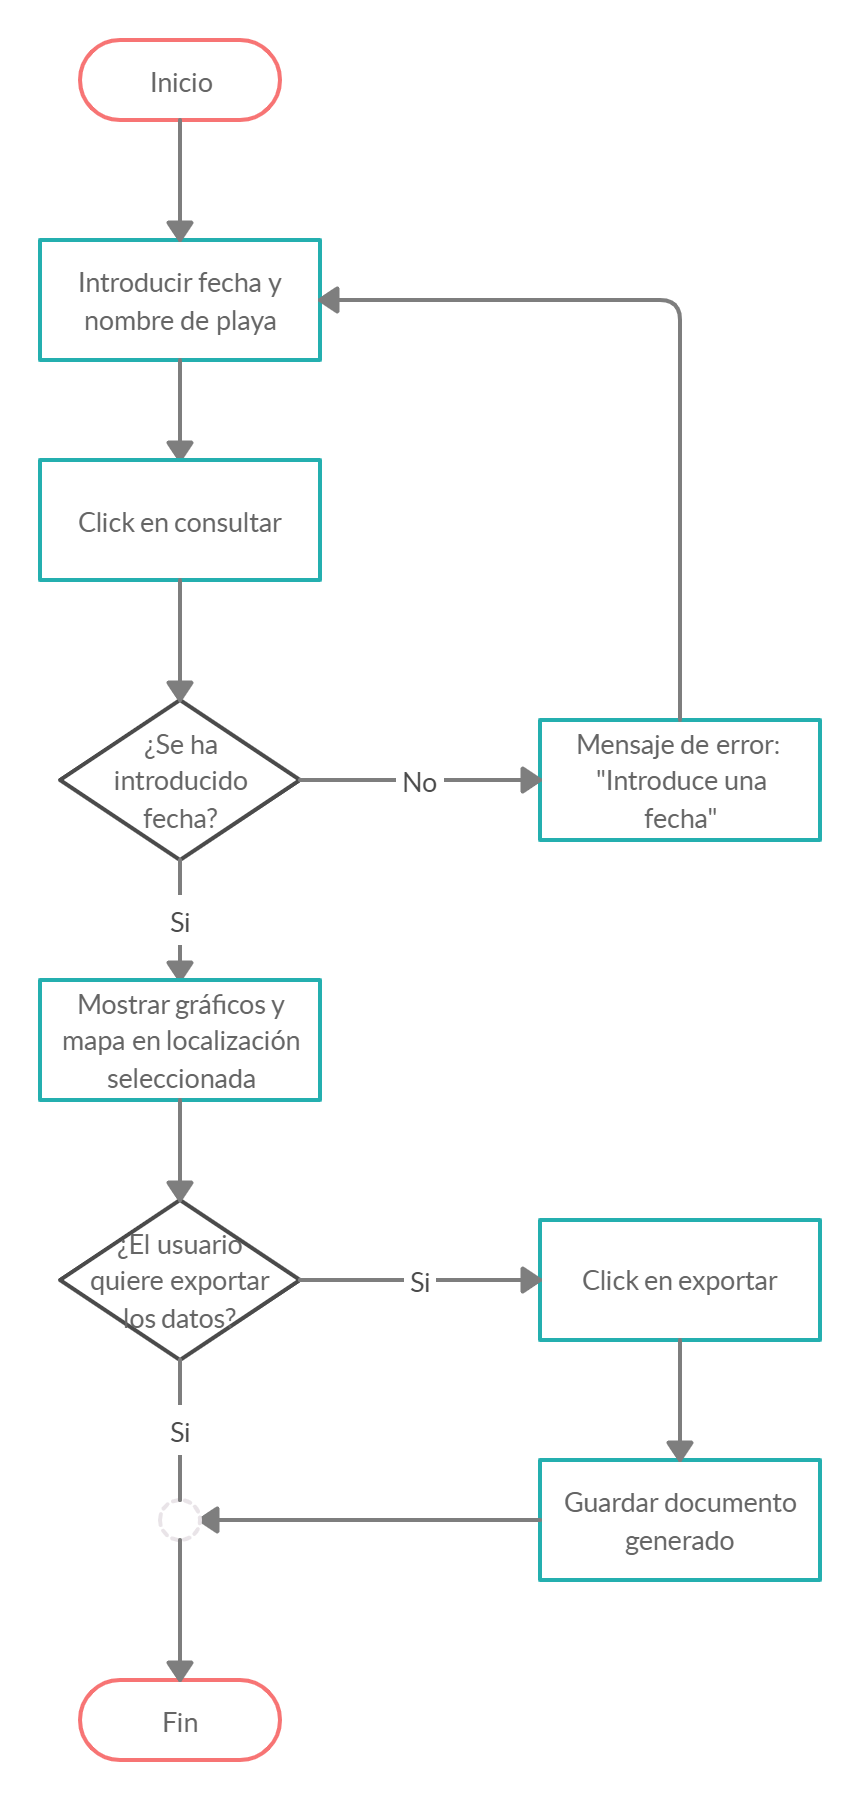
\includegraphics[width=0.6\textwidth]{diagramaFlujo.png}
	\caption{Diagrama de flujo}\label{fig:diagrama}
\end{figure}

\section{Diseño arquitectónico}

\textcolor{red}{PREGUNTAR MVC??}

\section{Diseño de interfaces}

Anteriormente a la realización de la aplicación, se realizaron una serie de bocetos en los que se reflejaron las principales ideas. Para esto se utilizó la aplicación Pencil.

\begin{figure}[!h]
	\centering
	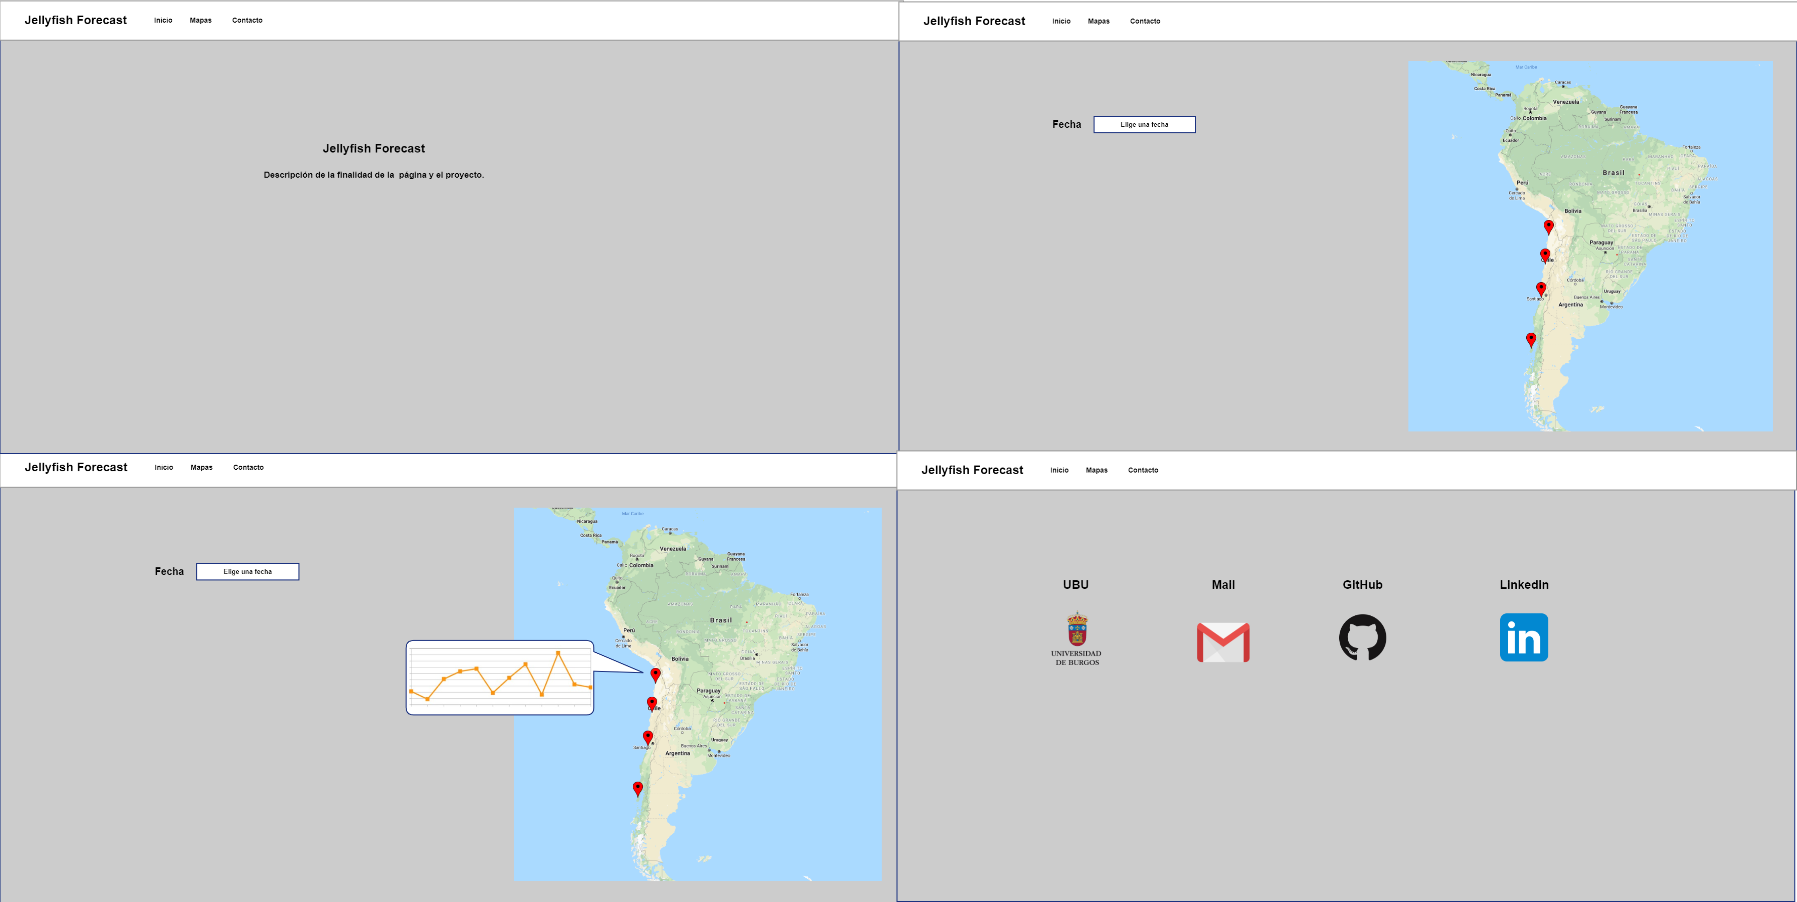
\includegraphics[width=1\textwidth]{bocetos.png}
	\caption{Bocetos iniciales}\label{fig:bocetos}
\end{figure}







